\documentclass[12pt]{article}
\usepackage{rotating}
\usepackage{graphicx, subfigure}
\begin{document}

\section{Exploratory Data Analysis}

\begin{figure}[ht!]
     \begin{center}
        \subfigure[]{
            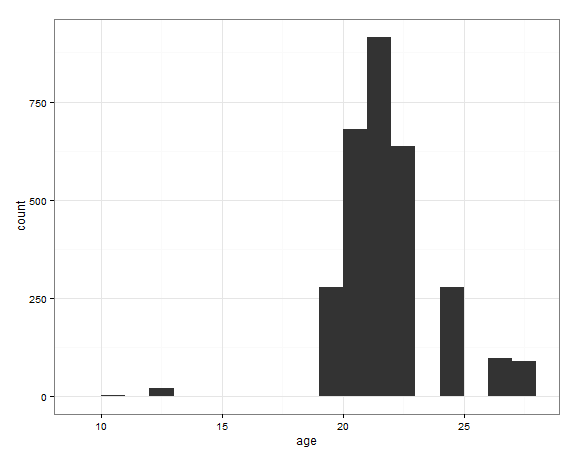
\includegraphics[width=0.45\textwidth]{../../output/demo_analysis/hist_age.png}
        }
        \subfigure[]{
           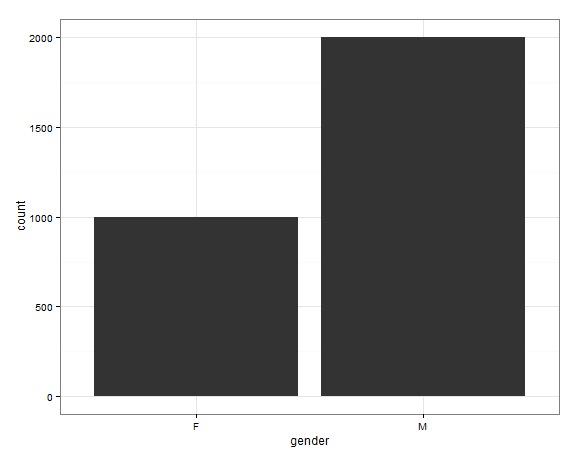
\includegraphics[width=0.45\textwidth]{../../output/demo_analysis/hist_gender.png}
		}
    \end{center}
    \caption{Histogram of age and gender of participants. }
\end{figure}

\begin{figure}[ht!]
     \begin{center}
        \subfigure[]{
            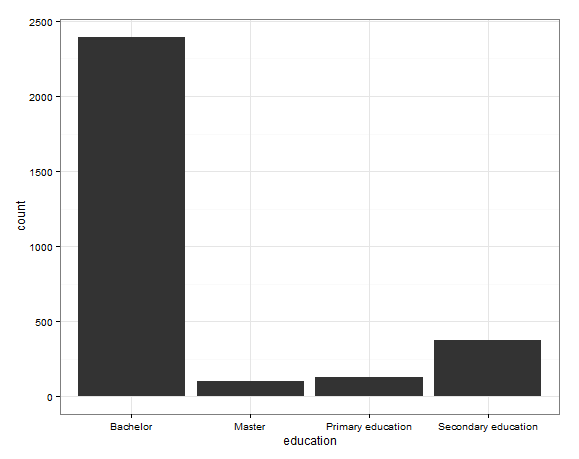
\includegraphics[width=0.45\textwidth]{../../output/demo_analysis/hist_edu.png}
      }
        \subfigure[]{
           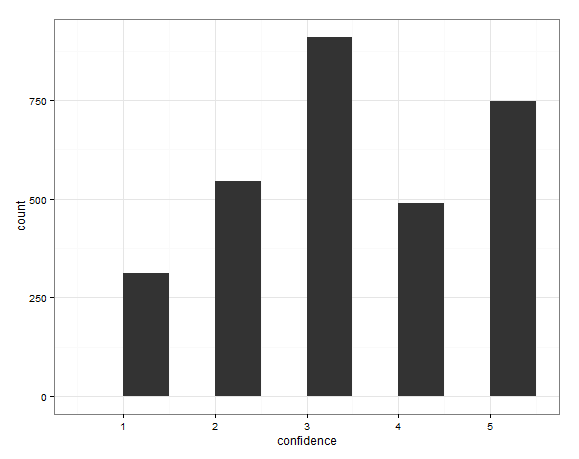
\includegraphics[width=0.45\textwidth]{../../output/demo_analysis/hist_confidence.png}
		}
    \end{center}
    \caption{Histogram of education level and confidence level. }
\end{figure}


\begin{figure}[ht!]
\begin{center}
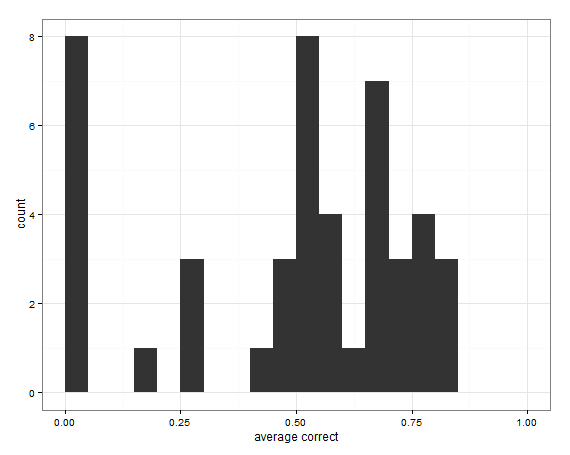
\includegraphics[width=0.45\textwidth]{../../output/demo_analysis/hist_user_perf_mc.png}
\caption{Histogram of user performance on multiple choice tasks.}
\end{center}	
\end{figure}


\begin{figure}[ht!]
     \begin{center}
        \subfigure[]{
            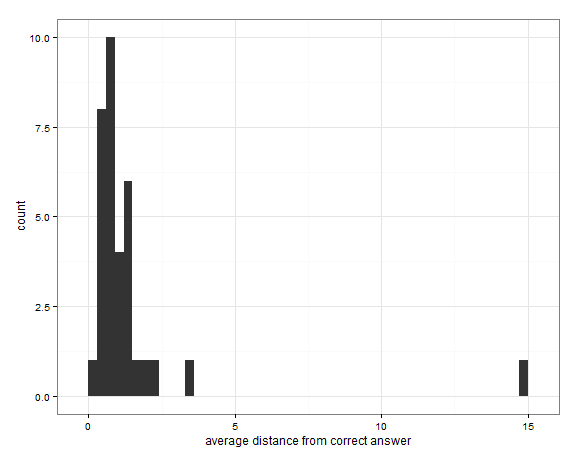
\includegraphics[width=0.45\textwidth]{../../output/demo_analysis/hist_user_perf_pe_tot.png}
        }
        \subfigure[]{
           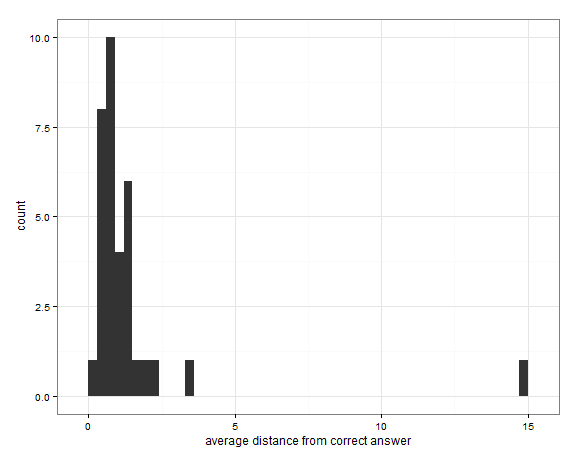
\includegraphics[width=0.45\textwidth]{../../output/demo_analysis/user_perf_pe_zoom.png}
		}
    \end{center}
    \caption{Histogram of aggregate user performance for point estimate tasks.}
\end{figure}


\begin{figure}[ht!]
\begin{center}
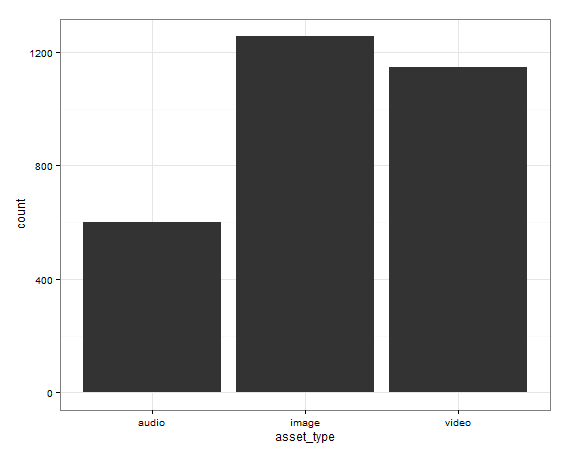
\includegraphics[width=0.45\textwidth]{../../output/demo_analysis/hist_assets.png}
\caption{Histogram of user performance on multiple choice tasks.}
\end{center}	
\end{figure}




\begin{figure}[ht!]
\begin{center}
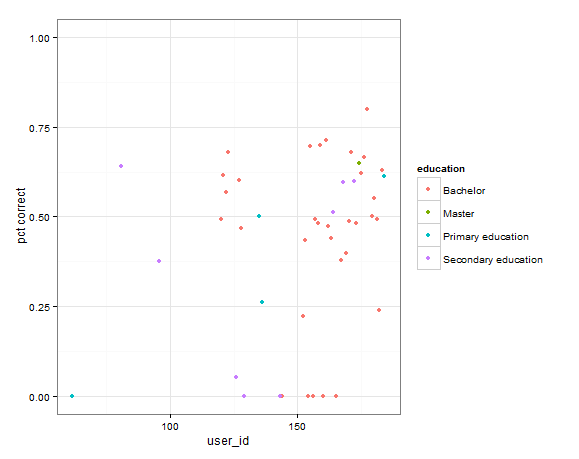
\includegraphics[width=0.45\textwidth]{../../output/demo_analysis/scatter_edu.png}
\caption{Scatter plot of accuracy by education level on multiple choice tasks.}
\end{center}	
\end{figure}


\begin{table}[ht!]
\centering
\begin{tabular}{rlr}
  \hline
 & type & av\_score \\ 
  \hline
1 & audio & 0.10 \\ 
  2 & image & 0.71 \\ 
  3 & video & 0.65 \\ 
   \hline
\end{tabular}
\caption{Average score by asset type for all domains.} 
\end{table}


\clearpage
\begin{table}[ht!]
\centering
\begin{tabular}{rlrr}
  \hline
 & education & pct\_correct & av\_dist \\ 
  \hline
1 & Bachelor & 0.42 & 1.46 \\ 
  2 & Master & 0.52 & 1.28 \\ 
  3 & Primary education & 0.45 & 1.22 \\ 
  4 & Secondary education & 0.40 & 1.42 \\ 
   \hline
\end{tabular}
\caption{Average score by education level all domains.} 
\end{table}

\begin{table}[ht]
\centering
\begin{tabular}{rrrr}
  \hline
 & confidence & pct\_correct & av\_dist \\ 
  \hline
1 &   1 & 0.23 & 1.35 \\ 
  2 &   2 & 0.17 & 1.50 \\ 
  3 &   3 & 0.31 & 1.33 \\ 
  4 &   4 & 0.52 & 2.01 \\ 
  5 &   5 & 0.75 & 0.66 \\ 
   \hline
\end{tabular}
\caption{Average score by confidence level all domains.} 
\end{table}


\begin{table}[ht]
\centering
\begin{tabular}{rlrr}
  \hline
 & asset\_type & av\_time & median\_time \\ 
  \hline
1 & audio & 18.04 & 16.00 \\ 
  2 & image & 12.26 & 11.00 \\ 
  3 & video & 17.73 & 17.00 \\ 
   \hline
\end{tabular}
\caption{Average and median time to answer question by asset type for all domains.} 
\end{table}


\begin{figure}[ht!]
     \begin{center}
        \subfigure[]{
            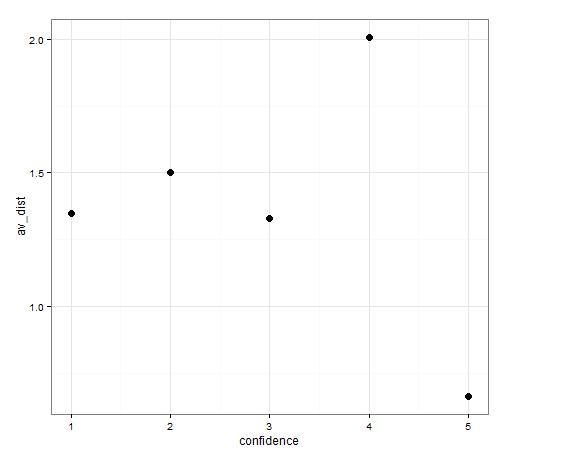
\includegraphics[width=0.55\textwidth]{../../output/demo_analysis/plot_conf_pe.png}
        }
        \subfigure[]{
           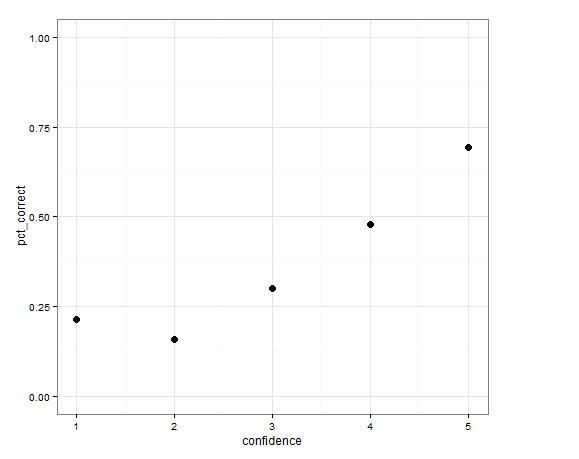
\includegraphics[width=0.55\textwidth]{../../output/demo_analysis/plot_conf_mc.png}
		}
    \end{center}
    \caption{Scatter plot of percent accuracy by reported confidence level for point estimate and multiple choice quesions. }
\end{figure}



\begin{figure}[ht!]
\begin{center}
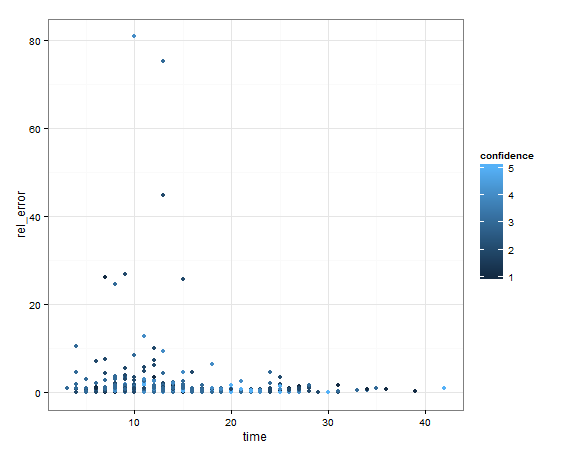
\includegraphics[width=0.65\textwidth]{../../output/demo_analysis/time_rel_error.png}
\caption{Relative Error vs time taken to answer question. Colour indicates reported confidence.}
\end{center}	
\end{figure}


\begin{table}[ht]
\centering
\begin{tabular}{rlr}
  \hline
 & experimental\_condition & time \\ 
  \hline
1 & control & 15.68 \\ 
  2 & social & 15.26 \\ 
   \hline
\end{tabular}
\caption{Average time to answer question by experimental condition.} 
\end{table}

\begin{table}[ht]
\centering
\begin{tabular}{rlrrr}
  \hline
 & experimental\_condition & av\_confidence & time & av\_score \\ 
  \hline
1 & control & 3.28 & 16.34 & 0.66 \\ 
  2 & social & 3.54 & 16.44 & 0.68 \\ 
   \hline
\end{tabular}
\caption{Statistics for experimental condition.} 
\end{table}

\begin{table}[ht]
\centering
\begin{tabular}{rrlrrrr}
  \hline
 & domain\_id & name & confidence & crowd\_score\_mc & crowd\_av\_error & crowd\_median\_err \\ 
  \hline
 &   3 & MagicTrick & 3.84 &  20 &  &  \\ 
 &   7 & Landmarks & 3.88 &  18 &  &  \\ 
 &  12 & Penalties & 2.75 &  12 &  &  \\ 
 &  19 & Calories & 2.75 &   & 1.43 & 0.69 \\ 
 &  53 & ThemeSongs & 2.82 &   4 &  &  \\ 
   \hline
\end{tabular}
\caption{Confidence vs domain error.} 
\end{table}

\clearpage

\section{Crowd Rankings}



\begin{table}[ht]
\centering
\begin{tabular}{rr}
  \hline
 & x \\ 
  \hline
domain & 19.00 \\ 
  abs\_error\_mean & 458.63 \\ 
  abs\_error\_median & 377.15 \\ 
  rel\_error\_mean & 1.43 \\ 
  rel\_error\_median & 0.69 \\ 
  rank\_mean & 0.45 \\ 
  rank\_median & 0.68 \\ 
  rank.geom.mean & 0.63 \\ 
  rank\_trunc\_mean & 0.58 \\ 
  rank\_trunc\_geom\_mean & 0.64 \\ 
   \hline
\end{tabular}
\caption{Point estimate domains ranked according to average ranking. Columns represent 
       the ranking by using the corresponding method of aggregation. Average ranking takes the 
       mean of the crowd percentiles for each task.} 
\end{table}



\begin{table}[ht]
\centering
\begin{tabular}{rrlrr}
  \hline
 & domain\_id & domain\_name & crowd\_score & crowd\_rank \\ 
  \hline
1 &   3 & MagicTrick & 20.00 & 1.00 \\ 
  2 &   7 & Landmarks & 18.00 & 0.92 \\ 
  3 &  12 & Penalties & 12.00 & 0.82 \\ 
  4 &  53 & ThemeSongs & 4.00 & 1.00 \\ 
   \hline
\end{tabular}
\caption{Multiple Choice domains. The Crowd Ranking column contains
       the percentage of users the crowd performs better than. 
       Score is the number of answers the crowd got right.} 
\end{table}




\begin{figure}[ht!]
     \begin{center}
        \subfigure[]{
            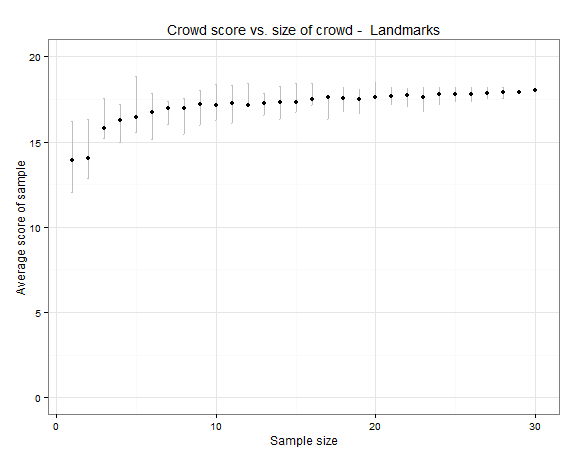
\includegraphics[width=0.55\textwidth]{../../output/demo_analysis/sample_size_landmarks.png}
        }
        \subfigure[]{
           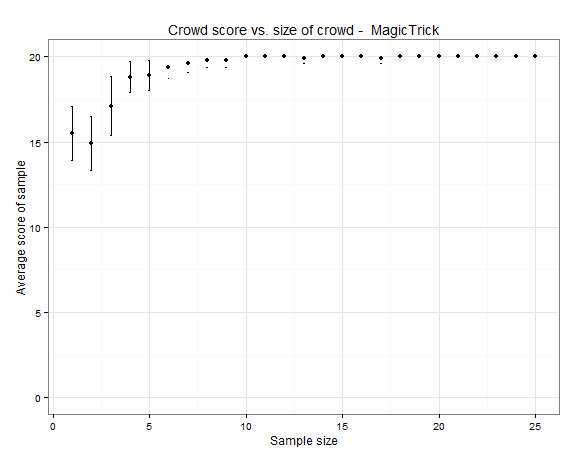
\includegraphics[width=0.55\textwidth]{../../output/demo_analysis/sample_size_magic.png}
		}
    \end{center}
    \caption{Sample size vs accuracy for landmarks (a) and magic trick (b).}
\end{figure}


\begin{figure}[ht!]
     \begin{center}
        \subfigure[]{
            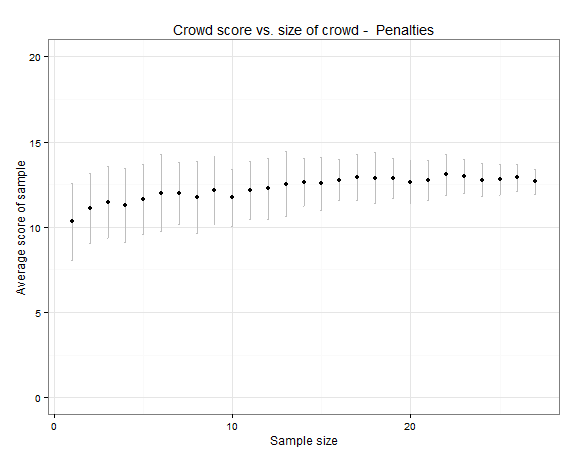
\includegraphics[width=0.55\textwidth]{../../output/demo_analysis/sample_size_penalties.png}
        }
        \subfigure[]{
           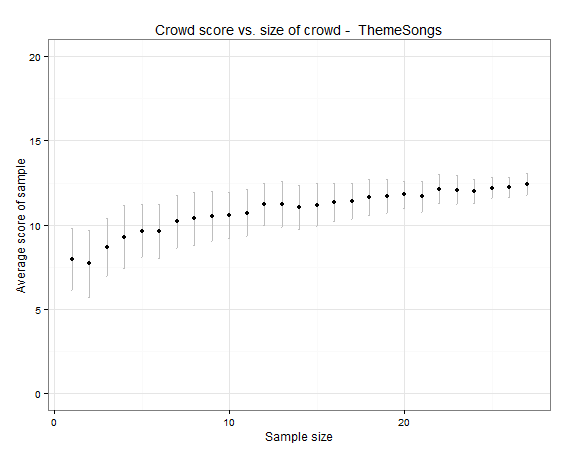
\includegraphics[width=0.55\textwidth]{../../output/demo_analysis/sample_size_themesongs.png}
		}
    \end{center}
    \caption{Sample size vs accuracy for penalties (a) and theme songs (b).}
\end{figure}



\begin{figure}[ht!]
\begin{center}
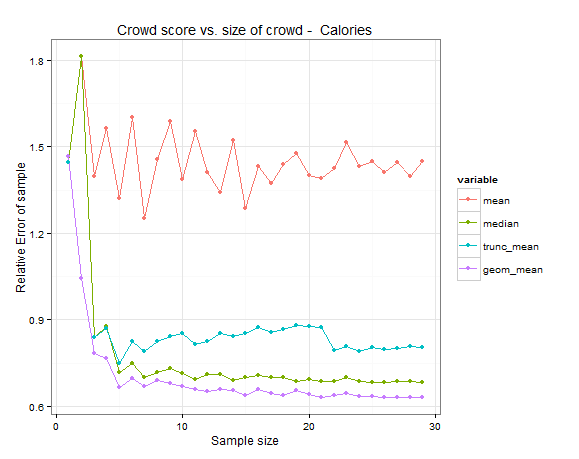
\includegraphics[width=0.95\textwidth]{../../output/demo_analysis/sample_size_calories.png}
\caption{Sample size vs accuracy for calories.}
\end{center}	
\end{figure}





\end{document}